\chapter{Konveks optimering}

Hvis et optimeringsproblem er konvekst, kan vi være sikre på at vi finner en global optimal løsning.

\section*{Definisjoner}

\begin{definition}{Lineært optimeringsproblem}{linear_programming}
  Et lineært optimeringsproblem er et optimeringsproblem på formen
  \begin{align*}
    \text{minimer}     & \quad \min_{x \in \R^n} f(x)                \\
    \text{betinget av} & \quad h_i(x) \leq 0, \quad i = 1, \ldots, m \\
                       & \quad g_j(x) = 0, \quad j = 1, \ldots, p
  \end{align*}
  hvor \(f, h_i, g_j\) er lineære funksjoner.
\end{definition}

\begin{example}{Lineær funksjon}{linear_function}
  La \(f(\symbf{x}) = c^T\symbf{x} + d\) være en lineær funksjon, hvor \(c\) er en vektor normal til en hyperplan og \(d\) er en konstant.
  Da er \(f(\symbf{x}) = 0\) en lineær likning som definerer en hyperplan i \(\R^n\).
\end{example}

\begin{example}{Lineær regresjon}{linear_regression}
  La \(X \in \R^{n \times m}\) være en matrise med observasjoner og \(y \in \R^n\) være en vektor med målinger.
  Lineær regresjon er et eksempel på et lineært program hvor vi ønsker å finne en vektor \(w \in \R^m\) som minimerer kvadratfeilen
  \begin{equation*}
    \min_{w \in \R^m} \norm{Xw - y}_2^2.
  \end{equation*}
\end{example}

\section[Slaters betingelse]{\gls{slater-condition}}

\begin{definition}{Slater's Condition}{slater_condition}
  For a convex problem with inequality constraints
  \[
    c_i(x) \le 0,\quad i=1,2,\dots,m,
  \]
  Slater's condition holds if there exists an \(x\) such that
  \[
    c_i(x) < 0 \quad \text{for all } i.
  \]
\end{definition}

\begin{remark}{Intuition}{}
  This condition guarantees that the feasible region has a nonempty interior.

  In other words, the constraints are not all 'tight' at every point, which helps secure strong duality and the existence of Lagrange multipliers.
\end{remark}

\section[KKT-betingelser]{\gls{kkt-conditions}}

\begin{theorem}{KKT conditions}{kkt}
  \begin{align*}
    \mathcal{A}_1(x)            & := \{i \in \mathcal{I} \mid c_i(x) = 0\},                     \\
    \mathcal{A}_2(x)            & := \{1 \leq i \leq m \mid (Ax)_i = b_i\} \tag{Active indices} \\
    \text{Active indices at } x & \in \Omega                                                    \\
  \end{align*}

  \begin{itemize}
    \item \(A_i\) are the active constraints/indices at \(x\)
    \item \(C\) is the matrix of equality constraints.
    \item \(p\) is the direction of descent.
    \item \(x\) is the current point (feasible).
    \item \(T_{\Omega}(x)\) is the tangent cone at \(x\).
    \item \(c_i(x)\) is the value of the \(i\)-th constraint at \(x\).
    \item \(Ax\) is the value of the equality constraints at \(x\).
    \item \(b\) is the vector of equality constraints.
  \end{itemize}

  Assume that \emph{Slater's constraint} holds. Then, the following statements are equivalent:

  \begin{align*}
    p\in T_{\Omega}(x) & \Longleftrightarrow
    \begin{cases}
      \inner{\nabla c_i(x), p} \geq 0, & i \in \mathcal{A}_1(x) \\
      (Ax)_i \geq 0,                   & i \in \mathcal{A}_2(x) \\
      Cp = 0,                          &                        \\
    \end{cases}
  \end{align*}

\end{theorem}


\begin{lemma}{Farka's Lemma}{farkas_lemma}
  Let \(A \in \mathbb{R}^{m \times n}\) and \(c \in \mathbb{R}^n\). Then, exactly one of the following statements is true:
  \begin{enumerate}
    \item[] \((1)\) There exists an \(x \in \mathbb{R}^n\) such that \(Ax \preceq 0\) and \(c^T x < 0\).
    \item[] \((2)\) There exists a \(y \in \mathbb{R}^m\) such that \(A^T y + c = 0\) and \(y \succeq 0\).
  \end{enumerate}
\end{lemma}

\begin{proof}
  \begin{enumerate}
    \item[] Assume that \((1)\) holds. Then \(Ax = b\) and \(x \ge 0\). If there exists a \(y\) such that \(y^T A \ge 0\), then
          \[
            y^T b = y^T Ax = (y^T A)x \ge 0,
          \]
          which contradicts \(y^T b < 0\).
    \item[] Assume that \((1)\) does not hold. We want to show that \((2)\) holds.

          Let
          \[
            K = \{Ax \mid x \ge 0\}.
          \]
          Since \((1)\) does not hold, \(b \notin K\). Since \(K\) is a closed convex cone, by the separating hyperplane theorem, there exists a \(y \in \mathbb{R}^m\) such that
          \[
            y^T b < y^T z \quad \text{for all } z \in K.
          \]
          Since \(0 \in K\), we have \(y^T b < 0\).

          Now, for any \(x \ge 0\), we have \(Ax \in K\), so \(y^T b < y^T Ax\).

          Let \(x = e_i\), where \(e_i\) is the \(i\)-th standard basis vector. Then \(x \ge 0\), and
          \[
            y^T A e_i = (y^T A)_i > 0.
          \]
          Thus \(y^T A \ge 0\).
  \end{enumerate}

  \begin{center}
    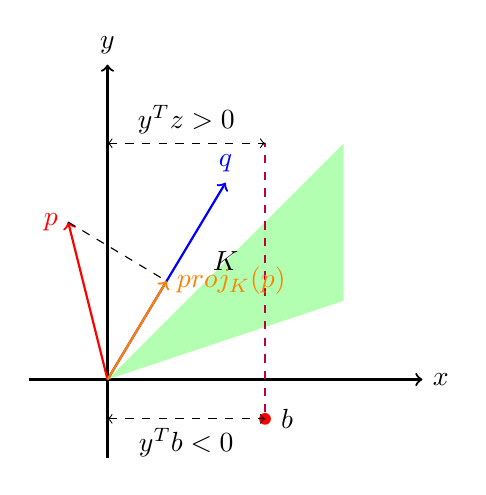
\begin{tikzpicture}
      \draw[->, thick] (-1, 0) -- (4, 0) node[right] {$x$};
      \draw[->, thick] (0, -1) -- (0, 4) node[above] {$y$};

      \fill[green!30] (0, 0) -- (3, 1) -- (3, 3) -- cycle;
      \node at (1.5, 1.5) {$K$};

      \node[circle, fill=red, inner sep=1.5pt, label=right:$b$] (b) at (2, -0.5) {};

      \draw[dashed, purple] (b) -- (2, 3);
      \draw[<->, dashed, black] (0, -0.5) -- (2, -0.5) node[midway, below, black] {$y^Tb < 0$};
      \draw[<->, dashed, black] (0, 3) -- (2, 3) node[midway, above, black] {$y^Tz > 0$};

      % Adding new vectors
      \draw[->, thick, blue] (0, 0) -- (1.5, 2.5) node[above] {$q$};
      \draw[->, thick, red] (0, 0) -- (-0.5, 2) node[left] {$p$};
      \draw[->, thick, orange] (0, 0) -- (0.75, 1.25) node[right] {$proj_K(p)$};
      \draw[dashed] (-0.5, 2) -- (0.75, 1.25);
    \end{tikzpicture}
  \end{center}

  The figure illustrates the geometric interpretation of Farkas' Lemma. The green region $K$ represents the cone of feasible points $\{Ax \mid x \ge 0\}$. The point $b$ (in red) lies outside this cone. The purple dashed line represents the separating hyperplane, which separates $b$ from $K$. Vector $p$ (in red) is projected onto the cone $K$, resulting in $proj_K(p)$ (in orange). Vector $q$ (in blue) lies inside the cone $K$. The black dashed lines show that the inner product $y^Tb$ is negative, while the inner product $y^Tz$ is positive for points $z$ in the cone $K$.

\end{proof}


\begin{theorem}{KKT conditions}{kkt_conditions}
  Assume \(c_i, i \in \mathcal{I}\) are concave in \(\mathcal{C}^1\),
  \(A\in \mathbb{R}^{m \times d}, b \in \mathbb{R}^m\) and \(C\in \mathbb{R}^{l \times d}\) and that \(f:\mathbb{R}^d \to \mathbb{R}\) is \(\mathcal{C}^1\). Assume that \emph{Slater's condition} holds.

  If \(x^\star\) is a local minimum of \(\min_x f(x)\) s.t.
  \[
    \begin{cases}
      c_i(x) \geq 0, & \forall i \in \mathcal{I} \\
      Ax \geq b,     &                           \\
      Cx = b,        &
    \end{cases}
  \]
  then there exists a \emph{Lagrange multipliers} \(\lambda^\star, \mu^\star\) with \(v \in \R^e\) s.t. the \emph{KKT conditions} hold:

  Then, the following statements are equivalent:
  \begin{align}
    \nabla f(x^\star) = \sum_{i\in \mathcal{I}} \lambda_i^\star \nabla c_i(x^\star) + A^T \mu^\star + C^T v^\star \\
    \begin{cases}
      c_i(x^\star) \geq 0, & \forall i \in \mathcal{I} \\
      Ax^\star \geq b,     &                           \\
      Cx^\star = e,        &                           \\
    \end{cases} \tag{Feasibility}                                                              \\
    \begin{cases}
      \lambda_i^\star \geq 0, & \forall i \in \mathcal{I} \\
      \mu_j^\star \in \geq 0, & \forall j \in \mathcal{J} \\
    \end{cases} \tag{Dual feasibility}                                                           \\
    \begin{cases}
      \lambda_i^\star c_i(x^\star) = 0, & \forall i \in \mathcal{I} \\
      \mu_j^\star C_j^T = 0,            & \forall j \in \mathcal{J} \\
    \end{cases} \tag{Complementary slackness}                                                 \\
    \begin{cases}
      \lambda_i^\star c_i(x^\star) = 0,      & \forall i \in \mathcal{I} \\
      \inner{\mu_j^\star, Ax^\star - b} = 0, & \forall j \in \mathcal{J} \\
    \end{cases} \tag{Complementary slackness}
  \end{align}
\end{theorem}

\begin{proof}{}{}
  We have the optimality condition:
  \[
    \inner{\nabla f(x^\star), p} \geq 0 \, \forall p \in T_{\Omega}(x^\star)
  \]
  \medskip
  \begin{align*}
    p \in T_{\Omega}(x^\star) \iff
    \begin{cases}
      \inner{\nabla c_i (x^\star), p }\geq 0 & \forall i \in \mathcal{A}_1(x^\star)                         \\
      \text{or: there does not exist any } p \in \R^d \text{ such that:} & \\
      \begin{cases}
        \inner{\nabla c_i (x^\star), p }\geq 0 & \forall i \in \mathcal{A}_1(x^\star) \\
        \inner{A_i^T , p }\geq 0               & \forall i \in \mathcal{A}_2(x^\star) \\
        \inner{ (C_i )^T, p } = 0              & \forall 1 \leq i \leq l              \\
        \inner{\nabla f (x^\star), p } < 0     & 
      \end{cases}                             \\
      (Ap)_i \geq 0 & \forall i \in \mathcal{A}_2(x^\star)                                                      \\
      Cp = 0        &
    \end{cases}
  \end{align*}

  The second alternative is Farka's Lemma does not hold \(\implies\) The first holds.

  \begin{align*}
    \nabla f(x^\star) & = \sum_{i\in \mathcal{A}_1(x^\star)} \lambda_i^\star \nabla c_i(x^\star) + \sum_{i \in \mathcal{A}_2(x^\star)} \mu_i^\star A_i^T + \sum_{i=1}^l v_i^\star C_i^T \\
  \end{align*}

  For some  \(\lambda_i^\star \geq 0, \mu_i^\star \geq 0, v_i^\star \in \R\).

  Now define: \(\lambda_i^\star = 0 \) for \(i \notin \mathcal{A}_1(x^\star)\) and \(\mu_i^\star = 0\) for \(i \notin \mathcal{A}_2(x^\star)\).

  Then we have:
  \begin{align*}
    \nabla f(x^\star) & = \sum_{i\in \mathcal{I}} \lambda_i^\star \nabla c_i(x^\star) + \sum_{1 \leq i \leq m} \mu_i^\star A_i^T + \sum_{1 \leq i \leq l} v_i^\star C_i^T = \text{(1)} \\
  \end{align*}
  \qed
\end{proof}

\begin{definition}{The Lagrangian of a problem}{lagrangian}
  The Lagrangian of a problem is the function \(\mathcal{L}: \mathbb{R}^d \times \mathbb{R}^m \times \mathbb{R}^l \times \mathbb{R}^e \to \mathbb{R}\) defined as:
  \begin{align*}
    \mathcal{L}(x, \lambda, \mu, v) &= f(x) + \sum_{i\in \mathcal{I}} \lambda_i c_i(x) + \sum_{1 \leq i \leq m} \mu_i (Ax - b)_i + \sum_{1 \leq i \leq l} v_i (Cx - b)_i \\
    &= f(x) - \sum_{i \in \mathcal{I}} \lambda_i c_i(x) - \inner{\mu, Ax - b} - \inner{v, Cx - e}\footnote{\( (1) \iff \nabla_x \mathcal{L}(x, \lambda, \mu, v) = 0\)}
  \end{align*}

\end{definition}